\documentclass{article}

\usepackage[letterpaper, margin=1.5cm]{geometry}

\renewcommand{\familydefault}{\sfdefault}

\usepackage[spanish]{babel}

\usepackage{graphicx}

\graphicspath{{./img/}}

\begin{document}

    \section*{Datos generales}

    \begin{itemize}
        \item Nombre: ISCX Botnet 2014 
        \footnote{https://www.unb.ca/cic/datasets/botnet.html}

        \item Nodos: 38499

        \item Enlaces: 41920

        \item Número de componentes conexas: 4

        \item Coeficiente de agrupamiento: 0.004

        \item Conectividad: 0

        \item Eficiencia local: 0.002663182752284772

        \item Densidad: 0.0000565671
    \end{itemize}

    \begin{figure}
        \centering
        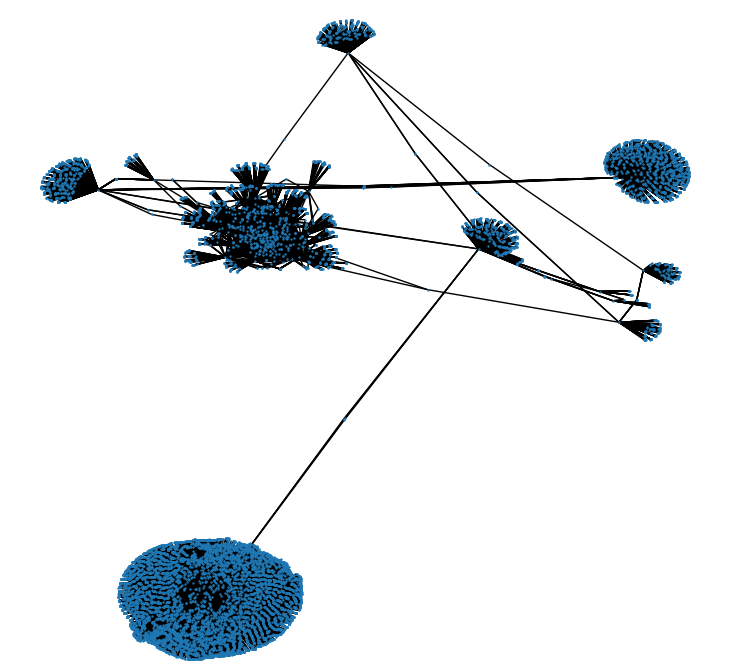
\includegraphics[scale=0.75]{net25.png}
        \caption{Red a estudiar con 25\% de los enlaces}
        \label{fig:net25}
    \end{figure}

    \begin{figure}
        \centering
        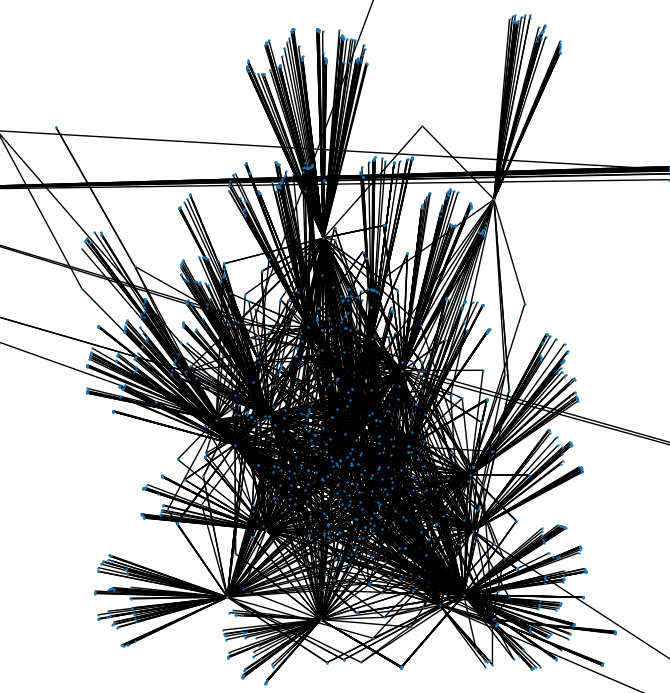
\includegraphics[width=\textwidth]{net25-detail.png}
        \caption{Detalle del componente gigante de la red a 25\%}
        \label{fig:net25detail}
    \end{figure}

    \begin{figure}
        \centering
        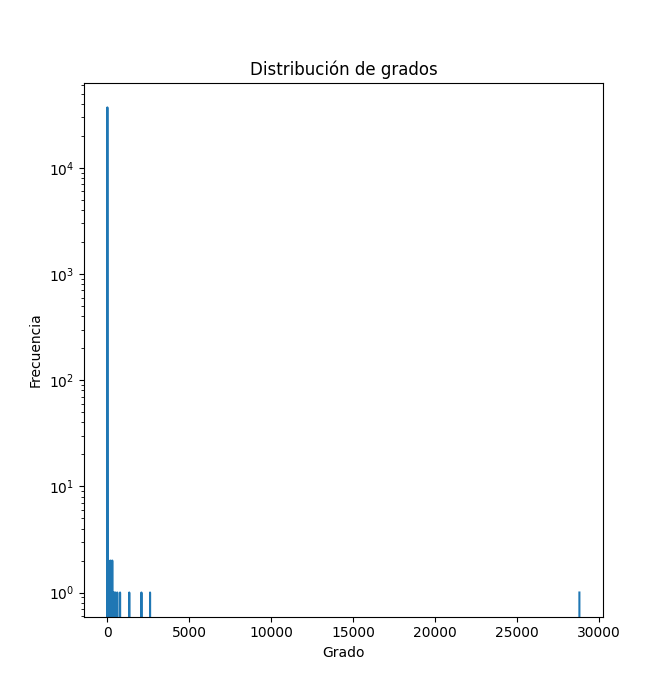
\includegraphics[scale=0.6]{degree_dist.png}
        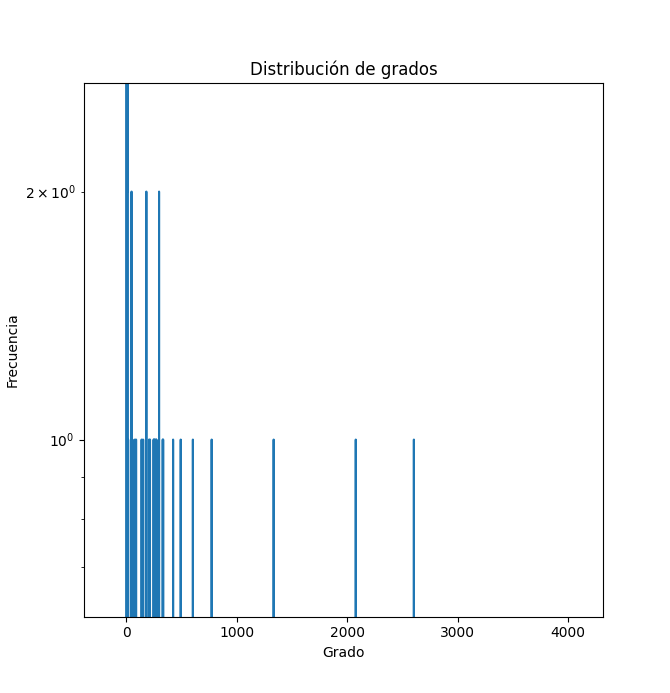
\includegraphics[scale=0.6]{degree_dist_detail.png}
        \caption{Distribución de grados. Dos escalas.}
        \label{fig:avgdeg}
    \end{figure}

    \begin{figure}
        \centering
        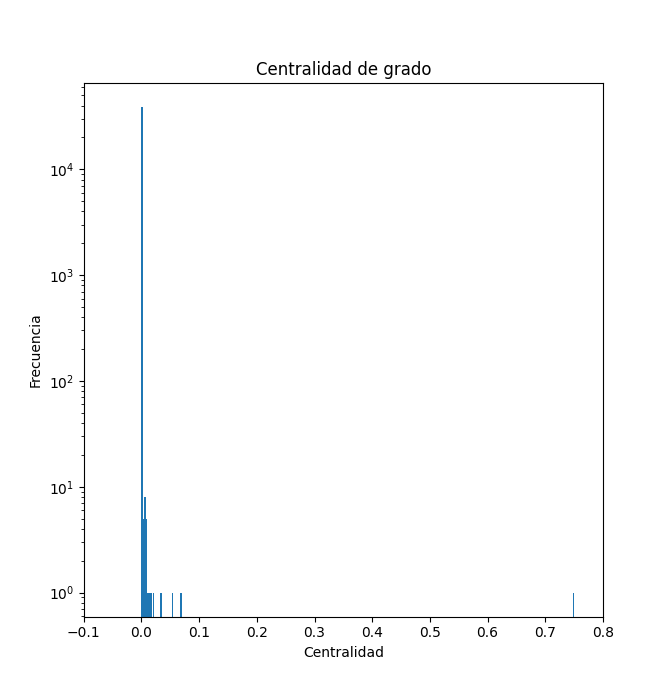
\includegraphics[scale=0.6]{degree_centrality.png}
        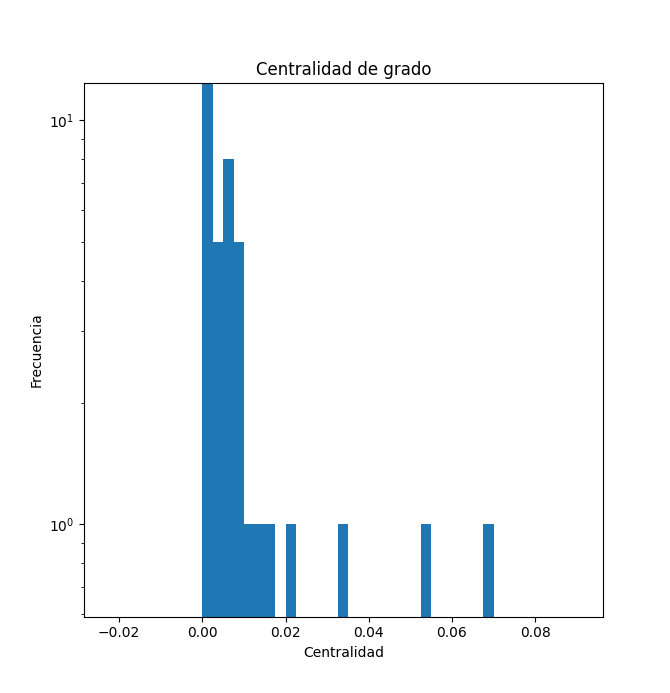
\includegraphics[scale=0.6]{degree_centrality_detail.png}
        \caption{Centralidad de grado. Dos escalas.}
        \label{fig:degcentr}
    \end{figure}

    \begin{figure}
        \centering
        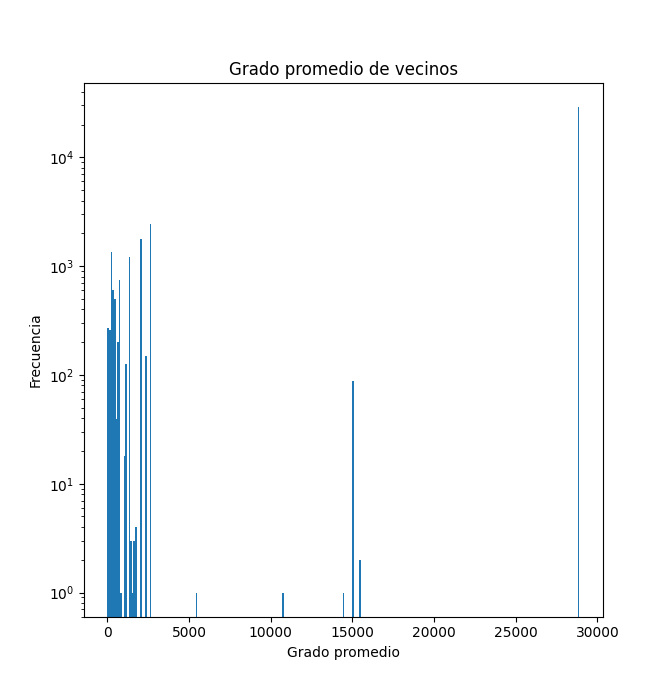
\includegraphics[scale=0.75]{avg_nei_degree.png}
        \caption{Grado promedio de vecinos}
        \label{fig:degeavgnei}
    \end{figure}

    \section*{Consideraciones}

    Varios de los datos estadísticos no sa han calculado debido a la cantida 
    necesaria de recursos para hacerlo.Se planea usar algún tipo de servicio 
    de computación distribuida para efectuar esos cálculos en el futuro.

    Se planea estudiar la componente gigante con  la estructura menos regular.

    Falta etiquetar los nodos infectados, así como incluir en el anális todo lo 
    relacionado a tiempo y evolución de la infección.
    
    En base a estos nuevos datos, se decidirá el modelo adecuado para modelar la
    red.
\end{document}